\chapter{Ultracold Quantum Gases in Optical Lattices}

Ultracold bosonic and fermionic quantum gases provide an incredible versatile tool in quantum research, as many novel quantum phenomena occur at extremely low temperatures. On of the most striking examples is a macroscopic population of the ground state of bosonic systems at sufficiently low temperatures, known as a Bose-Einstein condensate \cite{WiemanCornell1995}.

Neutral atoms in particular offer the unique feature of tunable collisional properties through Feshbach resonances, where any two-body scattering length can be achieved by applying a magnetic field \cite{Inouye1998,Zwierlein2004}. However, unlike for charged particles, magnetic traps can only trap a small subset of the available spin states of the neutral atoms \cite{Bloch2005}. Therefore, one must employ optical dipole traps, which utilize the interaction between an oscillating electric field and the induced dipole moment in the atoms to generate potentials \cite{grimm}. However, any scattering of the atoms off the electric field must be suppressed to maintain low temperatures, which is achieved through large detunings and high field intensities \cite{manybodyBloch}. Hence, lasers are required for creating optical potentials.

By overlapping counter-propagating laser beams, one can create periodic potentials known as \textit{optical lattices}. These types of potentials are extremely versatile, as they can be created in a multitude of different configurations. Furthermore, the periodic nature of the potential causes the emergence of energy spectra in the form of bands, which is otherwise known from condensed matter physics. Together with the tunable interactions from Feshbach resonances, a wide range of Hamiltonians can be mapped unto ultracold gases in optical lattices \cite{JakschZoller, Bloch2012}.\\

A weakly interacting bosonic gas trapped in an optical lattice a well described by a macroscopic wavefunction akin to a Bose-Einstein condensate. However, as the interaction strength grows, the system becomes increasingly correlated. A prominent example is the Bose-Hubbard model, describing bosons occupying the lowest Bloch band of a lattice. This model features a quantum phase transition between a weakly interacting superfluid phase and a strongly correlated Mott-insulator \cite{Fisher1989}. These two phases exhibit very different properties, as  particles are highly de-localized across the entire lattice in the superfluid phase, while the Mott is defined by zero compressibility, as the atoms are evenly distributed in the lattice. Several methods exist for deriving phase diagrams of the Bose-Hubbard model. Here, a mean-field approach is taken, as it provides a very intuitive picture of the model.


\section{Optical Lattice Potentials}
Cold atoms can be trapped in potentials generated by their own dipole interaction with light. Thus, superimposing laser beams allows one to create optical potentials in various shapes and forms. Such dipole traps realised using far-detuned light have important properties, as (i) they are capable of trapping neutral atoms, and (ii) the optical excitation from the trap is very low resulting in only small losses \cite{grimm}. Optical lattices are a central component of many experiments, as they not only trap the atoms, but also determine important properties of the system.

\subsection{Trapping of Neutral Atoms}
Consider a two level atom in the presence of a time-varying electric field
\begin{equation}
	\boldsymbol{E} = \boldsymbol{\varepsilon} E_0 \big( \exp \left( i(\boldsymbol{k} \boldsymbol{r} - \omega_L t) \right) + \mathrm{c.c.} \big) \; ,
\end{equation}
where $E_0$ is its amplitude, $\boldsymbol{\varepsilon}$ is its polarization vector, $\boldsymbol{k}$ is its wave vector and $\omega_L$ is its frequency. The interaction between the atom and the electric field causes a perturbation of the atoms energy levels, otherwise known as the ac-Stark shift. The Hamiltonian describing this interaction is
\begin{equation}
	\hat{H}_{int} = \hat{d} \cdot \boldsymbol{E} \; , \label{eq:Hdipint}
\end{equation}
where $\hat{d} = -e \hat{r}$ is the electric dipole operator \cite{greiner}.\\
The perturbative ac-Stark shift results in an effective dipole potential. This can be derived through the \textit{dressed state picture}, where the combined system of an atom and the light field is considered \cite{cohen1992atom,cohen1998}. Consider a two-level atom in the ground state $\ket{g}$ and a light field containing $n$ photons. The unperturbed energy of this state is $\varepsilon_g = n \hbar \omega_L$, where the ground state energy of the atom is merely an offset and therefore is discarded. The atom can become excited by absorbing one of the photons from the light field, whereby the unperturbed energy becomes $\varepsilon_e = \hbar \omega_0 + (n-1) \hbar \omega_L = - \hbar \Delta + n \hbar \omega_L$, where $\Delta = \omega_L - \omega_0$ is defined as the detuning. 

The coherent interaction between the atom and the light field can be determined through perturbation theory. This interaction is described by the Hamiltonian $\hat{H}_{int}$, and the strength of the interaction is much smaller than the energy level separation of the atom \cite{grimm}.
To first order the non-degenerate, time-independent perturbation of the energy of a state $i$ reads
\begin{equation}
	E_{i}^{(1)} = \bra{i} \hat{H}_{int} \ket{i} = 0\; ,
\end{equation}
which vanishes due to the symmetry of the interaction Hamiltonian.
To second order the perturbation of state $i$ is given by
\begin{equation}
	E_i^{(2)} = \sum_{j \neq i} \frac{ |\bra{j} \hat{H}_{int}\ket{i}|^2}{\varepsilon_i - \varepsilon_j} \; ,
\end{equation}
where $\varepsilon_i$ is the unperturbed energy of the $i$'th state. For a two-level atom, the only states contributing to the perturbation are $\ket{g}$ and $\ket{e}$ with $\varepsilon_g - \varepsilon_e = \hbar \Delta $. Therefore, the energy shift due to the coherent interaction between the atom and the light field becomes
\begin{equation}
	E_{g/e}^{(2)}= \pm  \frac{ |\bra{e}\hat{d}\ket{g}|^2}{\hbar \Delta} |E_0|^2,
	\label{2ndpert}
\end{equation}
where the plus and minus signs are associated with the ground and excited state respectively. Eq. \eqref{2ndpert} can be rewritten in order to reflect properties of the atom and the field, by considering the intensity of the light
\begin{equation}
	I = \frac{1}{2} \epsilon_0 c |\boldsymbol{E}|^2 \; ,
\end{equation}
and the decay rate of the atom \cite{grimm}
\begin{equation}
	\Gamma = \frac{\omega_{0}^3}{3 \pi \epsilon_0 \hbar c^3} |\braket{e | \hat{d} | g}|^2 \; .
\end{equation}
Thus, the energy shift experienced by the atom can be written as  
\begin{equation}
	E_{e/g}^{(2)}=\pm \frac{3 \pi c^2}{2 \omega_{0}^3} \frac{\Gamma}{\Delta}I \; .
	\label{eq:dipolepot}
\end{equation}
This is the AC-Stark shift, which constitutes the dipole potential. For red detuning ($\Delta < 0$) the ground state will experience a negative shift leading to an attractive potential with depth depending on the intensity of the laser. Oppositely, a blue-detuned laser ($\Delta > 0$) will repel the atom. An illustration of this can be seen in figure \ref{fig:ac_stark}.
\begin{figure}[!t]
	\centering
	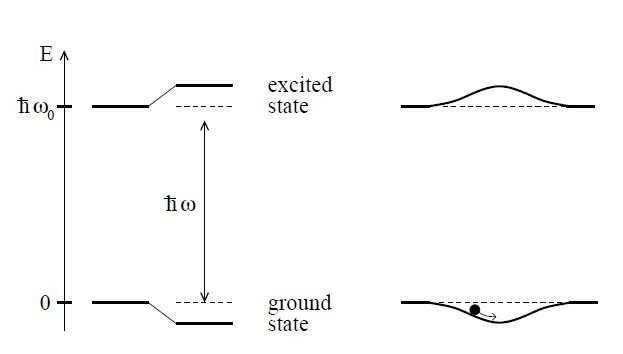
\includegraphics[width=0.5\columnwidth]{Figures/acstark.JPG} 
	\caption{\textit{Light shifts of a two-level atom. Left-hand side,
		red-detuned light ($\Delta < 0$) shifts the ground state down and the
		excited state up by same amounts. Right-hand side, a spatially
		inhomogeneous field like a Gaussian laser beam produces a
		ground-state potential well, in which an atom can be trapped. Figure and 		caption are adopted from \cite{grimm}.}}
	\label{fig:ac_stark} 
\end{figure}
Since the sign of the perturbation is reversed for the excited state, the effect of the detuning becomes opposite, whereby it is important that the atom remains in the ground state. Thus, one has to minimize the scattering with the optical potential. The scattering rate is given as \cite{grimm}
\begin{equation}
	\Gamma_{sc} = \frac{3 \pi c^2}{2 \hbar \omega_{0}^3}  \left( \frac{\Gamma}{\Delta} \right) ^2 I \; .
\end{equation}
As the detuning becomes small, the laser becomes resonant with the atom causing a large increase in scattered photons. Therefore, one has to choose a large detuning in order for the potential to remain conservative. However, this comes at the cost of a weaker potential. To compensate this, a high laser intensity must be used for the potential to reach sufficient depth. In practice there will be a limit to the laser power available, however, for most alkali-metal atoms the detuning is typically chosen to be large compared to the excited-state hyperfine structure splitting, which provides enough depth while sufficiently suppressing scattering events \cite{manybodyBloch}. 


\subsection{Optical Lattices}

The dipole potential in equation \eqref{eq:dipolepot} scales with the intensity of the laser. Thus, superimposing laser beams enables a multitude of different potentials through the interference patterns of the lasers. A standing wave from two counter-propagating light fields will lead to an array of potential wells
\begin{equation}
	V(z) = - V_0 \cos^2{k z } \; ,
	\label{eq:standwave}
\end{equation}
where $V_0 = | \frac{3 \pi c^2}{2 \omega_{0}^3} \frac{\Gamma}{\Delta} 4 I_0 |$ is derived from eq. \eqref{eq:dipolepot}. In practice, the one-dimensional lattice structure of eq. \eqref{eq:standwave} is created by shining a single laser beam at a mirror, whereby it interferes with itself.
\begin{figure}[!t]
	\centering
	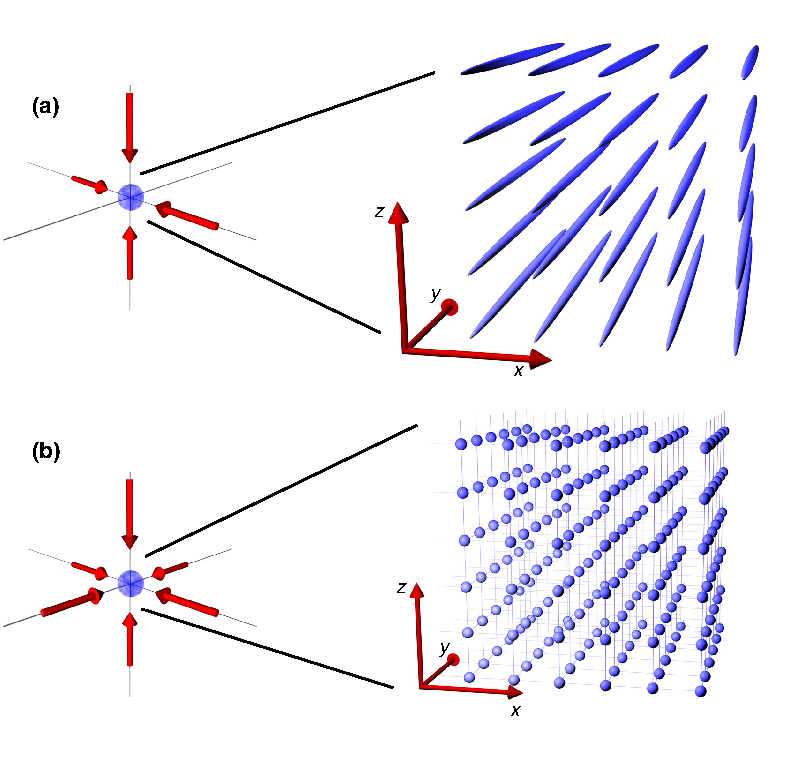
\includegraphics[width=0.7\columnwidth]{Figures/OpticalLattice.pdf} 
	\caption{\textit{\textbf{(a)} Two dimensional optical lattice formed by two mutually orthogonal laser beams. These tubes have a characteristic cigar shape, due to the Gaussian profile of the lasers. \textbf{(b)} Upon using three orthogonal laser beams, the result is a three dimensional lattice reminiscent of a cubic crystal. Figure is adopted from \cite{WideraThesis}.}}
	\label{fig:OpticalLattice} 
\end{figure}
Adding another standing laser beam in a different direction creates a periodic two dimensional potential. For orthogonal polarization of the two lasers, the resulting potential is purely the sum of the sinusoidal standing wave potential, as no interference term is present \cite{lewenstein}. Note, the lattice is only well defined for distances much smaller than the waist of the laser beams, as the lattice is only present within the overlap of the two beams. Various shapes of the lattice can be achieved by adjusting the angle between the beams, however, the most common setup is using two orthogonal beam creating a square lattice of one dimensional tubes, as seen in figure \ref{fig:OpticalLattice}(a).
In order to create a three dimensional lattice, as seen in figure \ref{fig:OpticalLattice}(b), an additional third perpendicular laser beam is needed. In the center of the trap, the lattice potential is then given by
\begin{equation}
	V(x,y,z) = - V_0 \left( \cos^2{k x } + \cos^2{k y } + \cos^2{k z } \right) \; , \label{eq:3Dlattice}
\end{equation}
for distances much smaller than the beam waist. In addition to the lattice, an external harmonic confinement will be present due to the Gaussian profile of the laser beams \cite{manybodyBloch}.

\subsection{Band Structure}
Consider a periodic potential as described by eq. \eqref{eq:standwave}. \textit{Bloch's Theorem} states that energy eigenstates of a periodic potential with lattice vector $\boldsymbol{R}$ and quasi-momentum $\boldsymbol{q}$ can be written as Bloch waves, which take the form
\begin{equation}
	\phi_{\boldsymbol{q}}^{(n)}(\boldsymbol{r}) = e^{i \boldsymbol{q} \boldsymbol{r}} u^{(n)}(\boldsymbol{r}) \; ,
\end{equation}
which is a plane wave modulated by a function with the same periodicity as the potential $u^{(n)}(\boldsymbol{r}) = u^{(n)}(\boldsymbol{r} + \boldsymbol{R})$. Furthermore, the Bloch waves are periodic in reciprocal space, such that $\phi_{\boldsymbol{q}}^{(n)}(\boldsymbol{r}) = \phi_{\boldsymbol{q} + \boldsymbol{G}}^{(n)}(\boldsymbol{r})$, where $\boldsymbol{G}$ is a reciprocal lattice vector \cite{kittel}.
This leads to an energy spectrum in the shape of bands with the periodicity of the first \textit{Brillouin Zone}. Bands are denoted by the band index $n$, and their shape is determined by both the shape and the depth of the potential. The potential depth is often denoted in units of the recoil energy $E_{\mathrm{rec}} = \frac{\hbar ^2 k^2}{2 m}$, where $m$ is the mass of the atom, and $k$ is the photon wave number of the light forming the optical lattice. For $V_0 = 0$, the particles are free, hence the bands will be parabolic. Meanwhile, for $V_0 \rightarrow \infty$, no interaction between different wells of the lattice can take place, as the wavefunctions of the trapped atoms will be confined to their respective well. Thus, the lattice is reduced to an array of independent harmonic oscillators, whereby the bands will appear flat with equal spacing \cite{greiner}. 

\subsection{Localized States}
The interaction strength between different lattice sites is determined by overlaps of the wavefunctions of the trapped atoms.
If the wavefunctions of one site only overlap with neighbouring wells, the lattice is considered being in the \textit{tight binding limit}. Thus, interactions between wells are almost purely of nearest neighbour nature. Due to how well localized the wavefunctions are, a basis of Wannier functions is ideal for describing the system. Wannier functions are related to Bloch functions through the Fourier transform \cite{kittel1963}
\begin{equation}
	w^{(n)}(\boldsymbol{r}) = \frac{1}{\sqrt{N_L}} \sum_{q} e^{ -i \boldsymbol{q} \boldsymbol{R} } \phi_{\boldsymbol{q}}^{(n)}(\boldsymbol{r}) \; ,
\end{equation} 
where $N_L$ is the number of primitive cells of the lattice. The Wannier functions are well localized and centered around the lattice at site $\boldsymbol{R}$. In the case of a separable periodic potential, like that of eq. \eqref{eq:3Dlattice}, the single-particle problem becomes one-dimensional \cite{kohn1959analyticWannier}. Lastly, Wannier functions obey the orthonormality relation
\begin{equation}
	\int \mathrm{d^3}r \; \; w^{(n) *}(\boldsymbol{r} - \boldsymbol{R}) w^{(n')}(\boldsymbol{r} - \boldsymbol{R'}) = \delta_{n,n'} \delta_{\boldsymbol{R},\boldsymbol{R}'} \; ,
\end{equation}
thus forming a complete basis \cite{manybodyBloch}. 
\begin{figure}[!h]
	\centering
	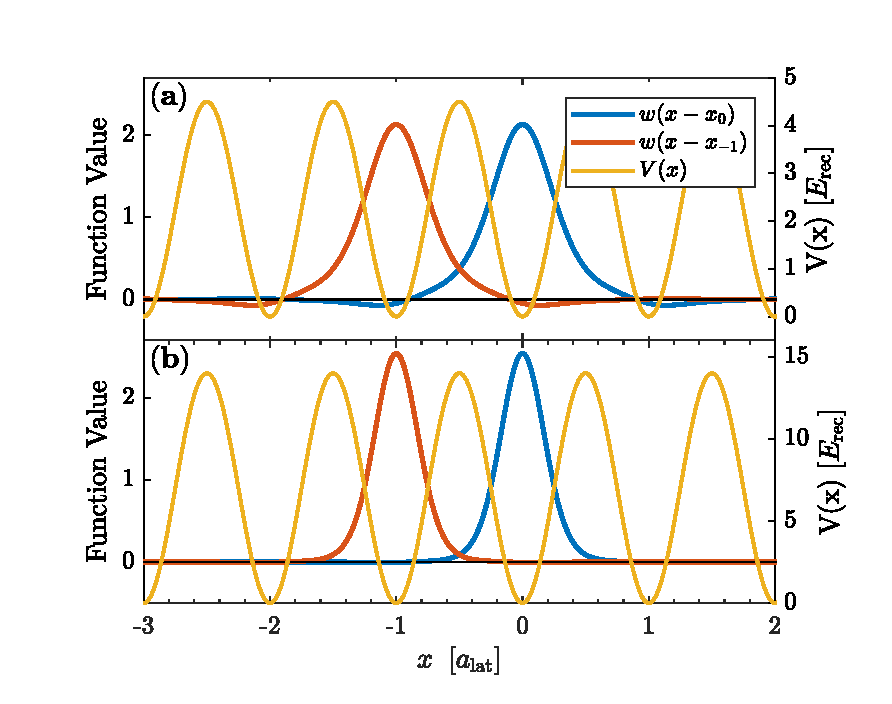
\includegraphics[width=0.8\columnwidth]{Figures/WannierFunctions.pdf} 
	\caption{Two one-dimensional Wannier functions plotted for lattice depths of \textbf{(a)} $V_0 = 4.5 E_{\mathrm{rec}}$ and \textbf{(b)} $V_0 = 14 E_{\mathrm{rec}}$.}
	\label{fig:WannierPlot} 
\end{figure}
Figure \ref{fig:WannierPlot}(a) shows Wannier functions plotted for lattice potential depths around the tight binding limit. As evident from the plot, the functions overlap with only their nearest neighbours. In the case of a more shallow lattice, the functions would extends to further wells, while they will tend towards a Gaussian shape as the lattice depth increases \cite{greiner}, which can be seen in figure \ref{fig:WannierPlot}(b).



\section{Bose-Einstein Condensates}

Bosons are particles of integer spin, whose statistics obey those of a Bose-Einstein distribution
\begin{equation}
	n_i = \frac{g_i}{\exp \left( \left( \varepsilon_i -\mu \right) / k_B T \right) - 1} \; , \label{eq:BHdistribution}
\end{equation} 
where $i$ denotes the state, $n_i$ is the population of the state, $g_i$ is its degeneracy, $\varepsilon_i$ is its energy, $\mu$ is the chemical potential, $k_B$ is the Boltzmann constant, and $T$ is the temperature. One important feature of bosons is that, unlike fermions, multiple particles can occupy the same quantum state. At higher temperatures the energy spectrum is practically continues, whereby this property has little effect, as two particles occupying the same single-particle state is highly unlikely. However, at low temperatures the energy spectrum systems become increasingly discrete, hence the statistics of the particles become very important. As evident from eq. \eqref{eq:BHdistribution}, the population of the ground state diverges as $T \to 0$. However, even below a finite temperature, $T_c$, one will observe a macroscopic population of the ground state. $T_c$ is called the critical temperature, and marks the point where multiple particles will start forming a Bose-Einstein Condensate (BEC). \cite{pethick2002bose}

\subsection{Non-Interacting Particles}
In the case of non-interacting particles and zero temperature, all particles of a Bose gas can be described by identical single-particles wavefunctions $\phi (\boldsymbol{r}_i)$. Hence, the many-body wavefunction is simply given by the product 
\begin{equation}
	\Psi (\boldsymbol{r}_1 , \ldots , \boldsymbol{r}_N) = \prod_{i}^{N} \phi (\boldsymbol{r}_i) \; .
\end{equation}
Such a product state can be described by a single macroscopic wavefunction
\begin{equation}
	\psi (\boldsymbol{r}) = \sqrt{N} \varphi (\boldsymbol{r}) \; , \label{eq:psi_NIBEC}
\end{equation}
where $\phi (\boldsymbol{r})$ is the wave function of the single-particle state, in which the bosons condensate into \cite{PenroseOnsager}.

\subsubsection{Second-Quantization}
When describing Bose-Einstein condensates it is very convenient to work in second quantization, which describes the number of particle in each state rather than the state of each particle.\\
First, consider a basis of single particle states $\{ \ket{n} \}$, namely a Fock basis. In this space particles are created or annihilated through their respective operators
\begin{equation}
	\hat{a}_{\mu}^{\dag} \ket{0}_\mu = \ket{1}_\mu \; .
\end{equation}
For bosons the creation and annihilation operators fulfill the commutation relations
\begin{equation}
[\hat{a}_\nu,\hat{a}_\mu]=[\hat{a}_\nu^\dagger,\hat{a}_\mu^\dagger]=0 \quad , \quad [\hat{a}_\nu,\hat{a}_\mu^\dagger]=\delta_{\nu,\mu} \; , 
\end{equation}
with the number operator given as
\begin{equation}
	\hat{n}_{\mu} = \hat{a}_{\mu}^{\dag} \hat{a}_{\mu} \; .
\end{equation}
In second quantization many-body states are described by the occupation of the individual Fock states. Thus, a creation operator will raise the number of particles in its corresponding state by one, while the annihilation operator will lower it:
\begin{align}
\hat{a}_{_\nu}^\dagger \ket{N_0,N_1, \ldots , N_{\nu},\ldots}&= \sqrt{N_\nu+1}\ket{N_0,N_1, \ldots , N_{\nu}+1,\ldots} \\
\hat{a}_{_\nu} \ket{N_0,N_1, \ldots , N_{\nu},\ldots}&= \sqrt{N_\nu}\ket{N_0,N_1, \ldots , N_{\nu}-1,\ldots} .
\end{align}
Likewise, the number operator $\hat{n}_{\mu}$ will count the number of particles in its corresponding state. These operators can be combined with an orthonormal basis of spatial wavefunctions $\{ \phi_k \}$ in order to create field operators
\begin{equation}
	\hat{\psi}(\boldsymbol{r}) = \; \sum_{k} \phi_k (\boldsymbol{r}) \hat{a}_{k} \quad , \quad \hat{\psi}^{\dag}(\boldsymbol{r}) = \; \sum_{k} \phi_{k}^{*} (\boldsymbol{r}) \hat{a}_{k}^{\dag} \; ,
\end{equation}
where $\hat{\psi}^{\dagger}(\boldsymbol{r})$ will create a particle at location $\boldsymbol{r}$. For bosons the field operators fulfill the commutation relations \cite{bruus}
\begin{equation}
	\left[ \hat{\psi}(\boldsymbol{r}) \; , \; \hat{\psi}^{\dag}(\boldsymbol{r'}) \right] = \; \delta^3(\boldsymbol{r} - \boldsymbol{r}') \quad , \quad
	\left[ \hat{\psi}(\boldsymbol{r}) \; , \; \hat{\psi}(\boldsymbol{r'}) \right] = \; 0 \; .
\end{equation}
Now, consider a gas of non-interacting bosons described by eq. \eqref{eq:psi_NIBEC}, where $\epsilon_k$ is the energy of the $k$'th single-particle state. Due to the completeness of the basis of single-particle wavefunctions, $\{ \phi_k \}$, the creation operator can be expressed as
\begin{equation}
	\hat{a}_{k}^{\dagger} = \int \mathrm{d^3} r \;  \phi_{k}^*(\boldsymbol{r}) \hat{\psi}^{\dagger}(\boldsymbol{r}) \; .
\end{equation}
Thereby the non-interacting Hamiltonian can be written as
\begin{align}
	\hat{H}^{(0)} =& \; \sum_{k} \epsilon_k \hat{a}_{k}^{\dag} \hat{a}_{k} \nonumber \\
		=& \;  \sum_{k} \int \mathrm{d^3}r_1 \mathrm{d^3}r_2 \; \epsilon_k \phi_k (\boldsymbol{r_2}) \phi_{k}^* (\boldsymbol{r_1})\;  \hat{\psi}^{\dag} (\boldsymbol{r_1}) \hat{\psi} (\boldsymbol{r_2}) \nonumber \\
		=& \; \int \mathrm{d^3}r  \; \hat{\psi}^{\dag}(\boldsymbol{r}) \left( - \frac{\hbar^2}{2 m} \nabla^2 + U(\boldsymbol{r})\right) \hat{\psi}(\boldsymbol{r}) \; ,
		\label{hamil2nd}
\end{align}
where the orthonormality of the wavefunctions
\begin{equation}
	\sum_{k}  \phi_k (\boldsymbol{r_2}) \phi_{k}^* (\boldsymbol{r_1}) = \delta^3(\boldsymbol{r_1} - \boldsymbol{r_2})
\end{equation} 
has been utilized.

\subsection{Weakly Interacting Particles}
A characteristic of a BEC is its low temperature and density. Thus, is it a valid approximation to only consider two-particle interactions
\begin{equation}
	\hat{H}^{(2)} = \frac{1}{2} \sum_{i \neq j} V(\boldsymbol{r_i} - \boldsymbol{r_j}) \; .
\end{equation}
At low energies all interactions can be considered of s-wave nature, because waves of higher angular momentum are reflected by the centrifugal barrier. Furthermore, the thermal de Broglie wavelength for cold gases is much larger than the effective extension of the interaction potential. Therefore, the actual shape of the scattering potential is irrelevant, whereby one can replace it with a pseudo-potential
\begin{equation}
	V(\boldsymbol{r} - \boldsymbol{r'}) = g \; \delta^3(\boldsymbol{r} - \boldsymbol{r'}) = \frac{4 \pi \hbar^2 a}{m} \delta^3(\boldsymbol{r} - \boldsymbol{r'}) \; ,
\end{equation}
which results in the same scattering phase as the real, more complicated scattering potential. Thus, the interaction of cold atoms is fully determined by the scattering length, $a$ \cite{greiner}.\\
Introducing the density operator
\begin{equation}
	\hat{\rho}(\boldsymbol{r}) = \hat{\psi}^{\dag}(\boldsymbol{r}) \hat{\psi}(\boldsymbol{r}) \; ,
\end{equation}
allows writing $\hat{H}^{(2)}$ in second quantization
\begin{align}
	\hat{H}^{(2)} &= \frac{1}{2} \int \mathrm{d^3}r_1 \mathrm{d^3}r_2 V(\boldsymbol{r_1} - \boldsymbol{r_2}) \hat{\psi}^{\dag}(\boldsymbol{r_1}) \hat{\psi}(\boldsymbol{r_1}) \left( \hat{\psi}^{\dag}(\boldsymbol{r_2}) \hat{\psi}(\boldsymbol{r_2}) - \delta(\boldsymbol{r_1} - \boldsymbol{r_2}) \right) \nonumber \\
	&= \frac{1}{2} \int \mathrm{d^3}r_1 \mathrm{d^3}r_2  \hat{\psi}^{\dag}(\boldsymbol{r_1}) \hat{\psi}^{\dag}(\boldsymbol{r_2}) V(\boldsymbol{r_1} - \boldsymbol{r_2}) \hat{\psi}(\boldsymbol{r_1}) \hat{\psi}(\boldsymbol{r_2}) \; .
\end{align}
Combining this with the basic Hamiltonian of equation \eqref{hamil2nd}, gives the full Hamiltonian in second quantization
\begin{align}
	\hat{H} &= \hat{H}^{(0)} + \hat{H}^{(2)} \\
	& = \int \mathrm{d^3}r \ \hat{\psi}^{\dag}(\boldsymbol{r}) \left( - \frac{\hbar^2}{2 m} \nabla^2 + U(\boldsymbol{r})\right) \hat{\psi}(\boldsymbol{r}) \nonumber \\
	 & \quad + \frac{1}{2} \int \mathrm{d^3}r_1 \mathrm{d^3}r_2  \ \hat{\psi}^{\dag}(\boldsymbol{r_1}) \hat{\psi}^{\dag}(\boldsymbol{r_2}) V(\boldsymbol{r_1} - \boldsymbol{r_2}) \hat{\psi}(\boldsymbol{r_1}) \hat{\psi}(\boldsymbol{r_2})
	\label{hamilint}
\end{align}
Solving the Heisenberg equations of motion using the field description of the Hamiltonian leads to
\begin{equation}
	i \hbar \frac{\partial }{\partial t} \hat{\psi}(\boldsymbol{r}) = \left[ \hat{\psi}(\boldsymbol{r}) \; , \; \hat{H}  \right] = \left( - \frac{\hbar^2}{2 m} \nabla^2 + U(\boldsymbol{r}) + g \hat{\psi}^{\dag}(\boldsymbol{r}) \hat{\psi}(\boldsymbol{r}) \right) \hat{\psi}(\boldsymbol{r}) \; ,
\end{equation}
which is not analytically solvable. However, if the scattering length $a$ is much less than the mean inter-particle distance, such that $n a^3 \ll 1$, where $n$ is the density of the gas, the mean-field approximation is viable
\begin{equation}
	\hat{\psi}(\boldsymbol{r}) = \psi(\boldsymbol{r}) + \delta \hat{\psi}(\boldsymbol{r}) \; ,
\end{equation}
where $\psi(\boldsymbol{r})$ is the mean-field given by eq. \eqref{eq:psi_NIBEC}, and $\delta \hat{\psi}(\boldsymbol{r})$ is fluctuations from the mean. If $\braket{\delta \hat{\psi}(\boldsymbol{r})} = 0$, the fluctuations can be neglected, leading to the Gross-Pitaevskii equation \cite{Gross1961,Pitaevskii}
\begin{equation}
	i \hbar \frac{\partial }{\partial t} \hat{\psi}(\boldsymbol{r}) = \left( - \frac{\hbar^2}{2 m} \nabla^2 + U(\boldsymbol{r}) + g |\psi(\boldsymbol{r})|^2 \right) \psi(\boldsymbol{r}) \; .
\end{equation}
The Gross-Pitaevskii equation is very similar to the Schrödinger equation with exception of the non-linear term $g |\psi(\boldsymbol{r})|^2$, which can make the equation hard to solve in regions of low density.



\section{Bose-Hubbard Model of Interacting Bosons in a Lattice} \label{sec:BHmodel}
The Bose-Hubbard model describes weakly interacting bosons in a periodic lattice within the tight binding limit. The model is perfectly capable of predicting results with good accuracy, however, two conditions must hold in order for it to be valid: (i) both the thermal energy and the mean interaction energy at a single site must be much smaller than the separation to first excited band, $\hbar \omega_0$, and (ii) the Wannier functions decay essentially within the length of the lattice constant \cite{manybodyBloch}.
Under these conditions one is assured that only the lowest band is taken into account, and that only nearest-neighbour interactions take place.

The Bose-Hubbard model is interesting, as it supports two distinct phases: The \textit{superfluid} phase and the \textit{Mott-insulator} phase. Furthermore, the model contains phenomena such as a quantum phase transition between the two phases mentioned above, which can be crossed without any change in external parameters.
While crossing the critical point, a state experiences a variety of quantum effects, which have great implications for the dynamics of the system.


\subsection{The Bose-Hubbard Hamiltonian}
Consider the Hamiltonian for bosonic particles in a trapping potential in one dimension as described by eq. \eqref{hamilint}. For a periodic lattice potential in the tight binding limit it is favourable to work in a basis of localized Wannier functions. Expanding the field operators of the Hamiltonian in eq. \eqref{hamilint} in  the Wannier basis yields \cite{Jaksch}
\begin{align}
	\hat{H} &= \int \mathrm{d}x \sum_{i j} w^*(x-x_i) \hat{a}_{i}^{\dag} \left( - \frac{\hbar^2}{2 m} \nabla ^2 + V(x) \right) w(x-x_j) \hat{a}_j \nonumber \\
	& \quad + g \int \mathrm{d}x \sum_{i j k l} w^*(x-x_i) w^*(x-x_j) w(x-x_k) w(x-x_l) \hat{a}_{i}^{\dag} \hat{a}_{j}^{\dag} \hat{a}_{k} \hat{a}_{l} \\
	&= - \sum_{i j } J_{i j} \hat{a}_{i}^{\dag} \hat{a}_{j} + \sum_{i j k l} U_{i j k l} \hat{a}_{i}^{\dag} \hat{a}_{j}^{\dag} \hat{a}_{k} \hat{a}_{l} \; ,
\end{align}
where
\begin{align}
	J_{i j} &= - \int \mathrm{d}x \ w^*(x-x_i) \left( - \frac{\hbar^2}{2 m} \nabla ^2 + V(x) \right) w(x-x_j) \label{eq:BHparamJ} \\
	U_{i j k l} &= g \int \mathrm{d}x \ w^*(x-x_i) w^*(x-x_j) w(x-x_k) w(x-x_l) 
\end{align}
Since the system is periodic, one can consider a single site, $i = 0$, as representative for the entire lattice. Thus, the different terms of the Hamiltonian can be interpreted as follows:
\begin{align}
	J_{0 0} &= \text{constant energy offset} \nonumber \\
	J_{0 1} &= \text{"overlap matrix element" to neighbouring site} \nonumber \\
	J_{0 2 - 0 \infty} &= \text{"overlap matrix element" to further sites} \nonumber \\
	U_{0 0 0 0} &= \text{on-site interaction for two particles} \nonumber \\
	U_{0 i i 0} &= \text{interaction off-site} \nonumber \\
	U_{0 0 0 1} &= \text{interaction  + tunnelling , off-site} \nonumber 
\end{align}
Due to the rapid decay of the Wannier functions, the overlap of wavefunctions is limited to their nearest neighbour. Dropping all exponentially suppressed terms and constant offsets yields the Bose-Hubbard Hamiltonian
\begin{equation}
	\hat{H} = - J \sum_{\langle i,j \rangle} \hat{a}_{i}^{\dag} \hat{a}_{j} + \frac{U}{2} \sum_{i} \hat{n}_i \left( \hat{n}_i -1 \right) + \sum_{i} \varepsilon_i \hat{n}_i \; ,
	\label{BHhamil}
\end{equation}
where $J = J_{0 1}$, the bracket $\langle i,j \rangle$ denotes only counting neighbouring pairs, and
\begin{equation}
	U = U_{0 0 0 0} = g \int \mathrm{d}x \ |w(x)|^4 \; .
	\label{eq:BHparamU}
\end{equation}
The first term of the Bose-Hubbard Hamiltonian describes the kinematics within the model, which takes the form of tunneling between neighbouring sites. This is interpreted by annihilating a particle at site $j$ while creating a particle at site $i$. The second term describes the interaction between particles within a single site, and the last term $\sum_{i} \varepsilon_i \hat{n}_i$ takes into account a possible potential offset at different sites.
\begin{figure}[!h]
	\centering
	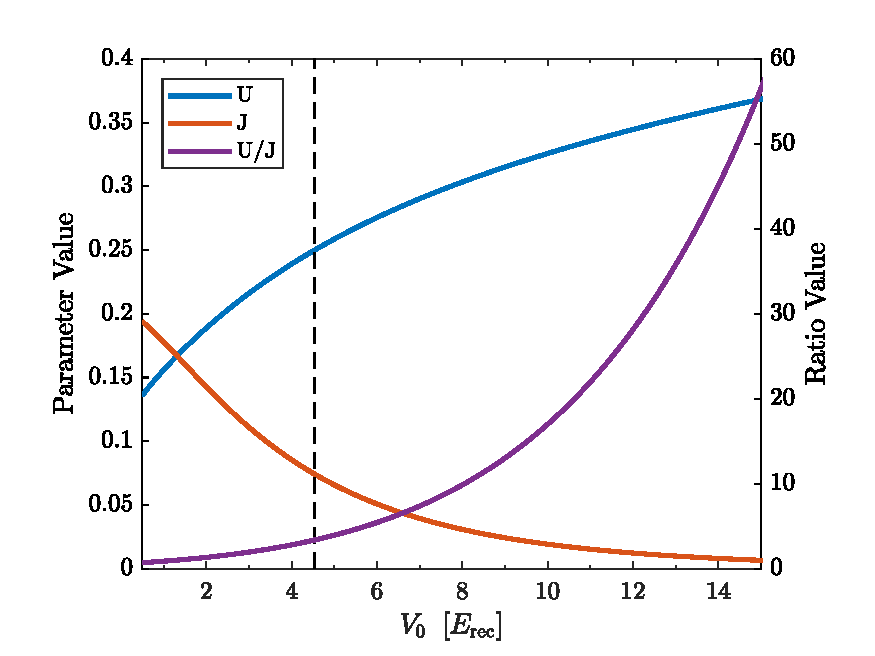
\includegraphics[width=0.8\columnwidth]{Figures/UJparameters.pdf} 
	\caption{Tunneling matrix element, $J$ \eqref{eq:BHparamJ}, and interaction strength, $U$ \eqref{eq:BHparamU}, as function of lattice depth. The parameters are calculated for Rubidium-87 atoms in an optical lattice with wavelength $\lambda = 1064 \mathrm{nm}$. The critical point of the Bose-Hubbard phase transition in one dimension is at $V_0 = 4.54 E_{\mathrm{rec}} \; , \; U/J = 3.37$ \cite{Kuhner2000}.}
	\label{fig:UJparameters} 
\end{figure}
Figure \ref{fig:UJparameters} illustrates the parameters of the Bose-Hubbard model as function of the lattice depth. The tunneling matrix element falls of very quickly with increasing lattice depth, as the Wannier functions become localized to their respective wells, thus reducing their overlap. The localization of the Wannier functions also causes the on-site interaction strength to increase.

\subsection{Phases of the Bose-Hubbard Model}

The Bose-Hubbard model supports two quantum phases: The \textit{superfluid} phase and the \textit{Mott-insulator} phase. These phases depend on the ratio $J/U$, and can be described separately by examining the ground state of the Bose-Hubbard Hamiltonian in the two extreme limits of the $J/U$ ratio.

\subsubsection{Superfluid Phase}
For a system where the tunneling matrix element $J$ is dominant, the lowest energy is obtained by delocalizing the atoms over the entire lattice. Thereby the wavefunction will be a product over single-particle states, and the system will be a superfluid \cite{greiner}.\\
Consider the case of negligible interactions and a lattice with wells of equal depth. In this scenario the Bose-Hubbard Hamiltonian reduces to
\begin{equation}
	\hat{H} = \hat{H}_J = - J \sum_{\langle i,j \rangle} \hat{a}_{i}^{\dag} \hat{a}_{j} \; , 
	\label{hamilSF}
\end{equation}
which is completely periodic within the lattice due to the lack of site specific terms. This leads to solutions in the shape of Bloch waves. The Fourier transform of the annihilation and creation operators reads
\begin{equation}
	\hat{a}_j = \frac{1}{L} \sum_{q}  e^{i q x_j} \hat{a}_q \quad , \quad
	\hat{a}_{j}^{\dag} = \frac{1}{L} \sum_{q}  e^{-i q x_j} \hat{a}_{q}^{\dag} \; ,
\end{equation}
where $L$ is the number of sites in the lattice. Through the Fourier transform the Hamiltonian \eqref{hamilSF} can be expressed in momentum space
\begin{equation}
	\hat{H}_J = - J \sum_{q = - \infty}^{\infty} \left( e^{- i q d } + e^{i q d} \right) \hat{n}_q \; ,
\end{equation}
where $d$ is the lattice distance. In momentum space the Hamiltonian \eqref{hamilSF} is diagonal and has a continuous energy spectrum
\begin{equation}
	E_q = -2 J \cos(q d) \; .
	\label{SFenergy}
\end{equation}
Thus, the excitation spectrum of the superfluid is said to be gapless. The lowest energy is of the system is obtained for $q = 0$, whereby the ground state is
\begin{equation}
	\ket{\Psi_{SF}} =  \frac{1}{\sqrt{N_{p} !}} \left( \hat{a}_{q = 0}^{\dag} \right) ^{N_{p}} \ket{0} = \frac{1}{\sqrt{N_{p} !}} \left( \frac{1}{L} \sum_{j = 1}^{L} \hat{a}_{j}^{\dag} \right) ^{N_{p}} \ket{0} \; ,
\end{equation} 
where $N_{p}$ is the number of particles. This state supports a well defined macroscopic phase on each lattice site, since the many-body state is a product over identical single-particle states \cite{greiner}. With all particles condensed into the $q = 0$ momentum space state, the particles are completely de-localized in real space, which can be seen by taking the Fourier transform. For large $N_{p} , L \rightarrow \infty$ at fixed density, $N_{p}/L$, the state becomes indistinguishable from having coherent states, $\ket{\alpha} $, on all lattice sites \cite{manybodyBloch}. Since bosonic operators at different sites commute, the superfluid state can be factorized into a product of local coherent states
\begin{equation}
	\ket{\Psi_{SF}} \approx \prod_j \left( e^{\sqrt{N_p/L} \hat{a}_{j}^{\dag}} \right) \ket{0} = \ket{\alpha_1} \otimes \ket{\alpha_2} \otimes \ldots
	\label{stateSF}
\end{equation}
\begin{figure}[!h]
	\centering
	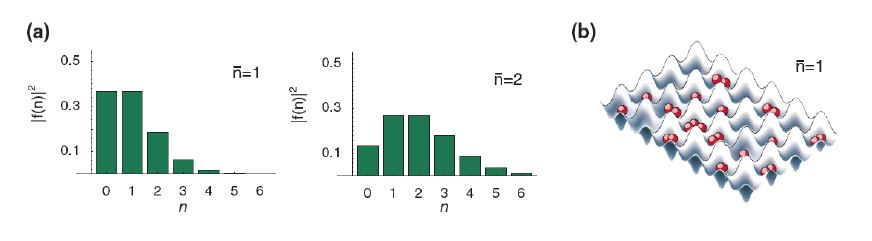
\includegraphics[width=0.8\columnwidth]{Figures/f(n)_SF.JPG} 
	\caption{\textbf{(a)} The statistics for the number of particles per lattice site $n$ for a filling fraction of $\bar{n}=1$ and $\bar{n}=2$ in the superfluid phase. \textbf{(b)} Illustration of the particles in the lattice. There will be large fluctuations of the number of particles found at each lattice site at a given time. Figure and caption adopted from \cite{greiner}.}
	\label{fig:f(n)_SF} 
\end{figure}
Coherent states are eigenstates of the annihilation operator $\hat{a} \ket{\alpha} = \alpha \ket{\alpha}$, where $|\alpha |^2$ can be considered the particle density of the system, and $\alpha = |\alpha| e^{i \phi}$, with $\phi$ being a global phase. Utilizing the coherent state form of the wavefunction \eqref{stateSF}, the average filling fraction $\bar{n}$ can be calculated
\begin{equation}
	\bar{n} = \braket{\hat{n}_i} = \bra{\Psi_{SF}} \hat{a}_{j}^{\dag} \hat{a}_{j} \ket{\Psi_{SF}} = \frac{N_p}{L} \; ,
\end{equation}
as well as the fluctuations of particle number per site
\begin{equation}
	\frac{\sqrt{\Delta \bar{n}^2}}{\bar{n}} \sim \frac{1}{\sqrt{\bar{n}}} \; .
\end{equation}
Therefore, the probability distribution for the number of atoms at a given site is Poissonian, which is illustrated in figure \ref{fig:f(n)_SF}. Due to the relatively large fluctuations of the particle number per site, one would find a somewhat random number of atoms at a given site in a single measurement. However, averaging over many measurements well produce the filling fraction $\bar{n}$. In the presence of a finite interaction the resulting distribution would be sub Poissonian due to number squeezing \cite{greiner}.


\subsubsection{Mott-Insulator Phase}
In the case of negligible tunneling, only the on-site interaction between the atoms has to be taken into account, and the Bose-Hubbard Hamiltonian reduces to
\begin{equation}
	\hat{H} = \hat{H}_U = \frac{U}{2} \sum_{i} \hat{n}_i \left( \hat{n}_i -1 \right) \; ,
	\label{hamilMott}
\end{equation}
which is quadratic in $\hat{n}_i$. This heavily penalizes having multiple particles at the same site. Thus, the ground state of the system will be an equal distribution of all the particles throughout the lattice. Any fluctuations from this average will increase the energy, whereby the phase is said to be incompressible \cite{Gemelke2009}. This incompressibility can be formulated as $\partial n / \partial \mu = 0$, where $\mu$ is the chemical potential, and is the defining property of the Mott-insulator \cite{manybodyBloch}.\\
\begin{figure}[!h]
\centering
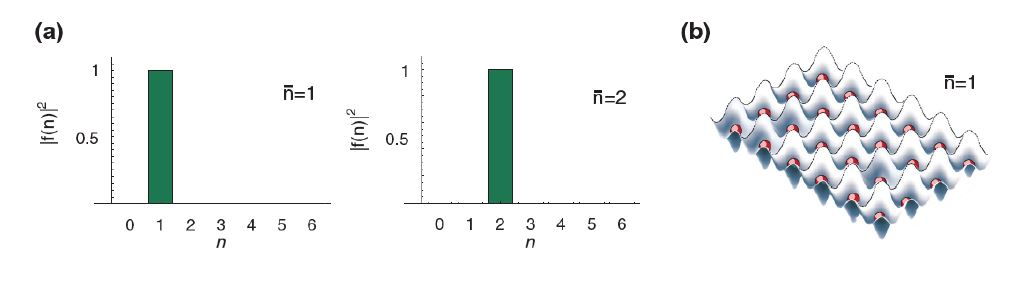
\includegraphics[width=0.8\columnwidth]{Figures/f(n)_M.JPG} 
\caption{\textbf{(a)} The statistics for the number of particles per lattice site $n$ in the Mott-insulator phase, for a filling fraction of $\bar{n}=1$ and $\bar{n}=2$. \textbf{(b)} Illustration of the particles in the lattice. The particles do not hop around in the lattice and are equally distributed. Caption and figure are adapted from \cite{greiner}.}
\label{fig:f(n)_M} 
\end{figure}
Consider the case of average filling of one particle per site, $\bar{n} = 1$. The many-body state can be described by a product of single particles located on each site \cite{manybodyBloch}
\begin{equation}
	\ket{\Psi_{Mott}} = \prod_j \hat{a}_{j}^{\dag} \ket{0} \; .
	\label{eq:MIstate}
\end{equation}
Eq. \ref{eq:MIstate} is a simple product of local Fock states with precisely one atom per site, which is illustrated in figure \ref{fig:f(n)_M}. This configuration of atoms minimizes the energy with regards to the interaction Hamiltonian \eqref{hamilMott}. Any fluctuation from unit occupancy will increase the energy, as a single double occupancy will increase the energy by $U$. Therefore, unlike the energy spectrum of the superfluid, the Mott-insulator spectrum is gapped. As long as the gain in kinetic energy due to hopping, $J$, is smaller than the on-site interaction, $U$, the atoms remain localized. However, for $J > 0$ the ground state is no longer the product state described in eq. \eqref{eq:MIstate} \cite{manybodyBloch}. As $J$ increases, the gap in the excitation spectrum will gradually decrease until the transition to the superfluid is reached and the spectrum becomes gapless.\\
While the Mott-insulator phase has complete localization, the phases on the individual sites have obtained maximum uncertainty. Therefore, no phase coherence between different sites is present \cite{greiner}.


\subsection{Mean-Field Approximation of Phase Diagram} \label{sec:MeanFieldDiagram}
Consider once again the full Bose-Hubbard Hamiltonian \eqref{BHhamil}. The superfluid and the Mott-insulator account for the two limits of the ratio $J/U$. However, in order to understand the full phase diagram of the Bose-Hubbard model, one has to derive the critical fraction $(J/U)_{crit}$ for which the phase transition occurs. There are several ways of doing this - one of them is looking at a mean-field solution of the Bose-Hubbard model. For simplicity the zero temperature case is treated here. Even without a change of temperature the phase transition still happens, hence it is referred to as a \textit{quantum phase transition}, since the phase transition can happen without change of external parameters \cite{Sachdev2007QPT}.

Applying the mean field approximation to the annihilation operator yields
\begin{equation}
	\hat{a}_j = \psi + \delta \hat{a}_j \; ,
\end{equation}
where $\psi$ is the locally constant mean field, and $\delta \hat{a}_j$ is the fluctuation term. Inserting this into the Bose-Hubbard Hamiltonian yields
\begin{equation}
	\hat{H}_{MF} = -J \sum_{\langle i,j \rangle} \left( \psi^* + \delta \hat{a}_{i}^{\dag} \right) \left( \psi + \delta \hat{a}_{j} \right) + \hat{H}_U
\end{equation}
Instead of considering the Hamiltonian as a whole, it can be considered as a sum of local on-site Hamiltonians
\begin{equation}
	\hat{H}_{MF} = \sum_{i} \hat{h}_i \; .
\end{equation}
For a homogeneous system, one can express the kinetic part of the Hamiltonian locally if only small fluctuations from the mean field are assumed
\begin{align}
  \hat{a}_{i}^{\dag} \hat{a}_{j} &= \left( \psi^* + \delta \hat{a}_{i}^{\dag} \right) \left( \psi + \delta \hat{a}_{j} \right) \nonumber \\
  &= \psi^* \psi + \psi^* \delta \hat{a}_j + \psi \delta \hat{a}_{i}^{\dag} + \delta \hat{a}_{i}^{\dag} \delta \hat{a}_{j} \nonumber \\
  & \approx \psi^* \psi + \psi^* \left( \hat{a}_j - \psi \right) + \psi \left( \hat{a}_{i}^{\dag} - \psi^* \right) \nonumber \\
&= \psi^* \hat{a}_j + \psi \hat{a}_{i}^{\dag} - \psi^* \psi \; .
\end{align}
Since every term contains only a single index, one can let $j \rightarrow i$ whereby
\begin{equation}
	\hat{h}_i = J z \psi^* \psi - J z \left( \psi^* \hat{a}_i + \psi \hat{a}_{i}^{\dag} \right) + \frac{U}{2} \hat{n}_i \left( \hat{n}_i -1 \right) + \mu_i \hat{n}_i \; ,
	\label{localhamil}
\end{equation}
where $z$ is the number of neighbours of site $i$ \cite{vanoosten}. The last term of eq. \eqref{localhamil} is a chemical potential, which had been added due to the lack of a fixed local particle number thereby prompting the use of a Grand Canonical Ensemble description.

Landau theory is a general theory regarding phase transitions, which states that in the vicinity of a critical point, one may expand the free energy in a power series of some order parameter. Here, the order parameter is the mean field, hence
\begin{equation}
	E_{MF} = \text{const.} + a |\psi|^2 + b |\psi|^4 + \ldots \label{eq:landau}
\end{equation} 
Eq. \eqref{eq:landau} constitutes an effective potential, which dictates certain properties of the system.
The potential is symmetric in the complex plane, whereby the Hamiltonian is invariant under $a \to a \; e^{-i \phi}$, for some phase $\phi$. Furthermore, at some critical value of $a$, (here $a = 0$), the potential will shift from having a single central minimum to having minima at some finite $|\psi|$. This is a U(1) spontaneous symmetry breaking, which in Landau theory is associated with a phase transition \cite{plischke}. Thus, one need to compute the parameter $a$ of equation \eqref{eq:landau}.

One method is using second order perturbation theory, where the $\hat{\psi} = 0$ case is solved exactly, followed by adding a small $\hat{\psi}$ as a perturbation. The zeroth order of the local mean-field Hamiltonian reads
\begin{equation}
	\hat{h}_{i}^{(0)} =  \frac{U}{2} \hat{n}_i \left( \hat{n}_i -1 \right) - \mu \hat{n}_i \; .
\end{equation} 
Since the zero-order solution contains only number operators, the ground state of the solution can be expressed in the Fock basis:
\begin{equation*}
\ket{\mathrm{gs}}_i = 
\begin{dcases}
   \ket{0} , & \text{for $\mu < 0$} \\
   \ket{1} , & \text{for $0 \leq \mu < U$} \\
   \ket{2} , & \text{for $U \leq \mu < 2 U$} \\
   & \vdots
\end{dcases}
\end{equation*}
Meanwhile, the perturbation Hamiltonian contains factors of the mean field 
\begin{equation}
	\delta \hat{h}_i = J z \left( \psi^* \psi \right) -   J z \left( \hat{a}_i \psi^* + \psi \hat{a}_{i}^{\dag} \right) \; .
\end{equation}
The goal is to find an expression for the parameter $a$, which determines the critical point. Thus, one must utilize up to second-order perturbation theory, as $a$ is the pre-factor of the contributions proportional to $|\psi|^2$. Since Fock states are orthogonal, all first order perturbations of the type $\braket{n | \hat{a}_i | n}$ vanish. Thus, the only first order contributions are 
\begin{equation}
	E_{i}^{(1)} = \bra{n} \delta \hat{h}_i \ket{n} = J z \left( \psi^* \psi \right)  \; .
\end{equation}
Next, the second order perturbations read
\begin{equation}
	E_{i}^{(2)} = \sum_{n \neq m} \frac{|\bra{n} \delta \hat{h}_i \ket{m}|^2}{E_{m}^{(0)} - E_{n}^{(0)}} \; .
\end{equation}
Since the local perturbation Hamiltonian contains single creation/annihilation operators, most contributions to the perturbation vanish as
\begin{equation}
	\bra{n} \delta \hat{h}_i \ket{m} = 0 \quad \text{for} \quad |n - m| \neq 1 \; .
\end{equation}
Thus, all the second order contributions origin from off-diagonal matrix elements reading
\begin{align*}
	\bra{n}  \hat{a}_{i}^{\dag} \ket{n-1} &= \sqrt{n} \braket{n|n} \\
	\bra{n+1}  \hat{a}_{i}^{\dag} \ket{n} &= \sqrt{n+1} \braket{n|n} \\
	& \vdots
\end{align*}
Summing all the contributions, the second order perturbation energy reduces to
\begin{align}
	E_{i}^{(2)} &= \left( J z \right)^2 |\psi|^2 \left( \frac{n}{E_{n}^{(0)}- E_{n-1}^{(0)}} +  \frac{n+1}{E_{n}^{(0)}- E_{n+1}^{(0)}} \right) \nonumber \\
	&= \left( J z \right)^2 |\psi|^2 \left( \frac{n}{U(n-1) - \mu} + \frac{n+1}{\mu - U n} \right) \; .
\end{align}
From eq. \eqref{eq:landau}, the scalar $a$ is the pre-factor of all terms proportional $|\psi|^2$. Collecting all terms from the perturbations yields the approximation 
\begin{equation}
	a = J z + \left( J z \right)^2 |\psi|^2 \left( \frac{n}{U(n-1) - \mu} + \frac{n+1}{\mu - U n} \right) \; .
\end{equation} 
As stated earlier $(J/U)_{crit}$ can be found at the point where $a = 0$, hence
\begin{equation}
	0 \overset{!}{=} 1 + \frac{n}{\bar{U} (n-1) - \bar{\mu}} + \frac{n+1}{\bar{\mu} - \bar{U} n} \; ,
\end{equation}
with $\bar{\mu} = {\mu}/{J z}$ and $\bar{U} = {U}/{J z}$. Finally, the solution for the chemical potential of eq. \eqref{localhamil} is \cite{vanoosten}
\begin{equation}
	\bar{\mu}_{\pm} = \frac{1}{2} \left( \bar{U}(2n -1) \pm \frac{1}{2} \sqrt{\bar{U}^2 - 2 \bar{U} (2 n +1)} \right) \; .
\end{equation}
 
\begin{figure}[h]
	\centering
	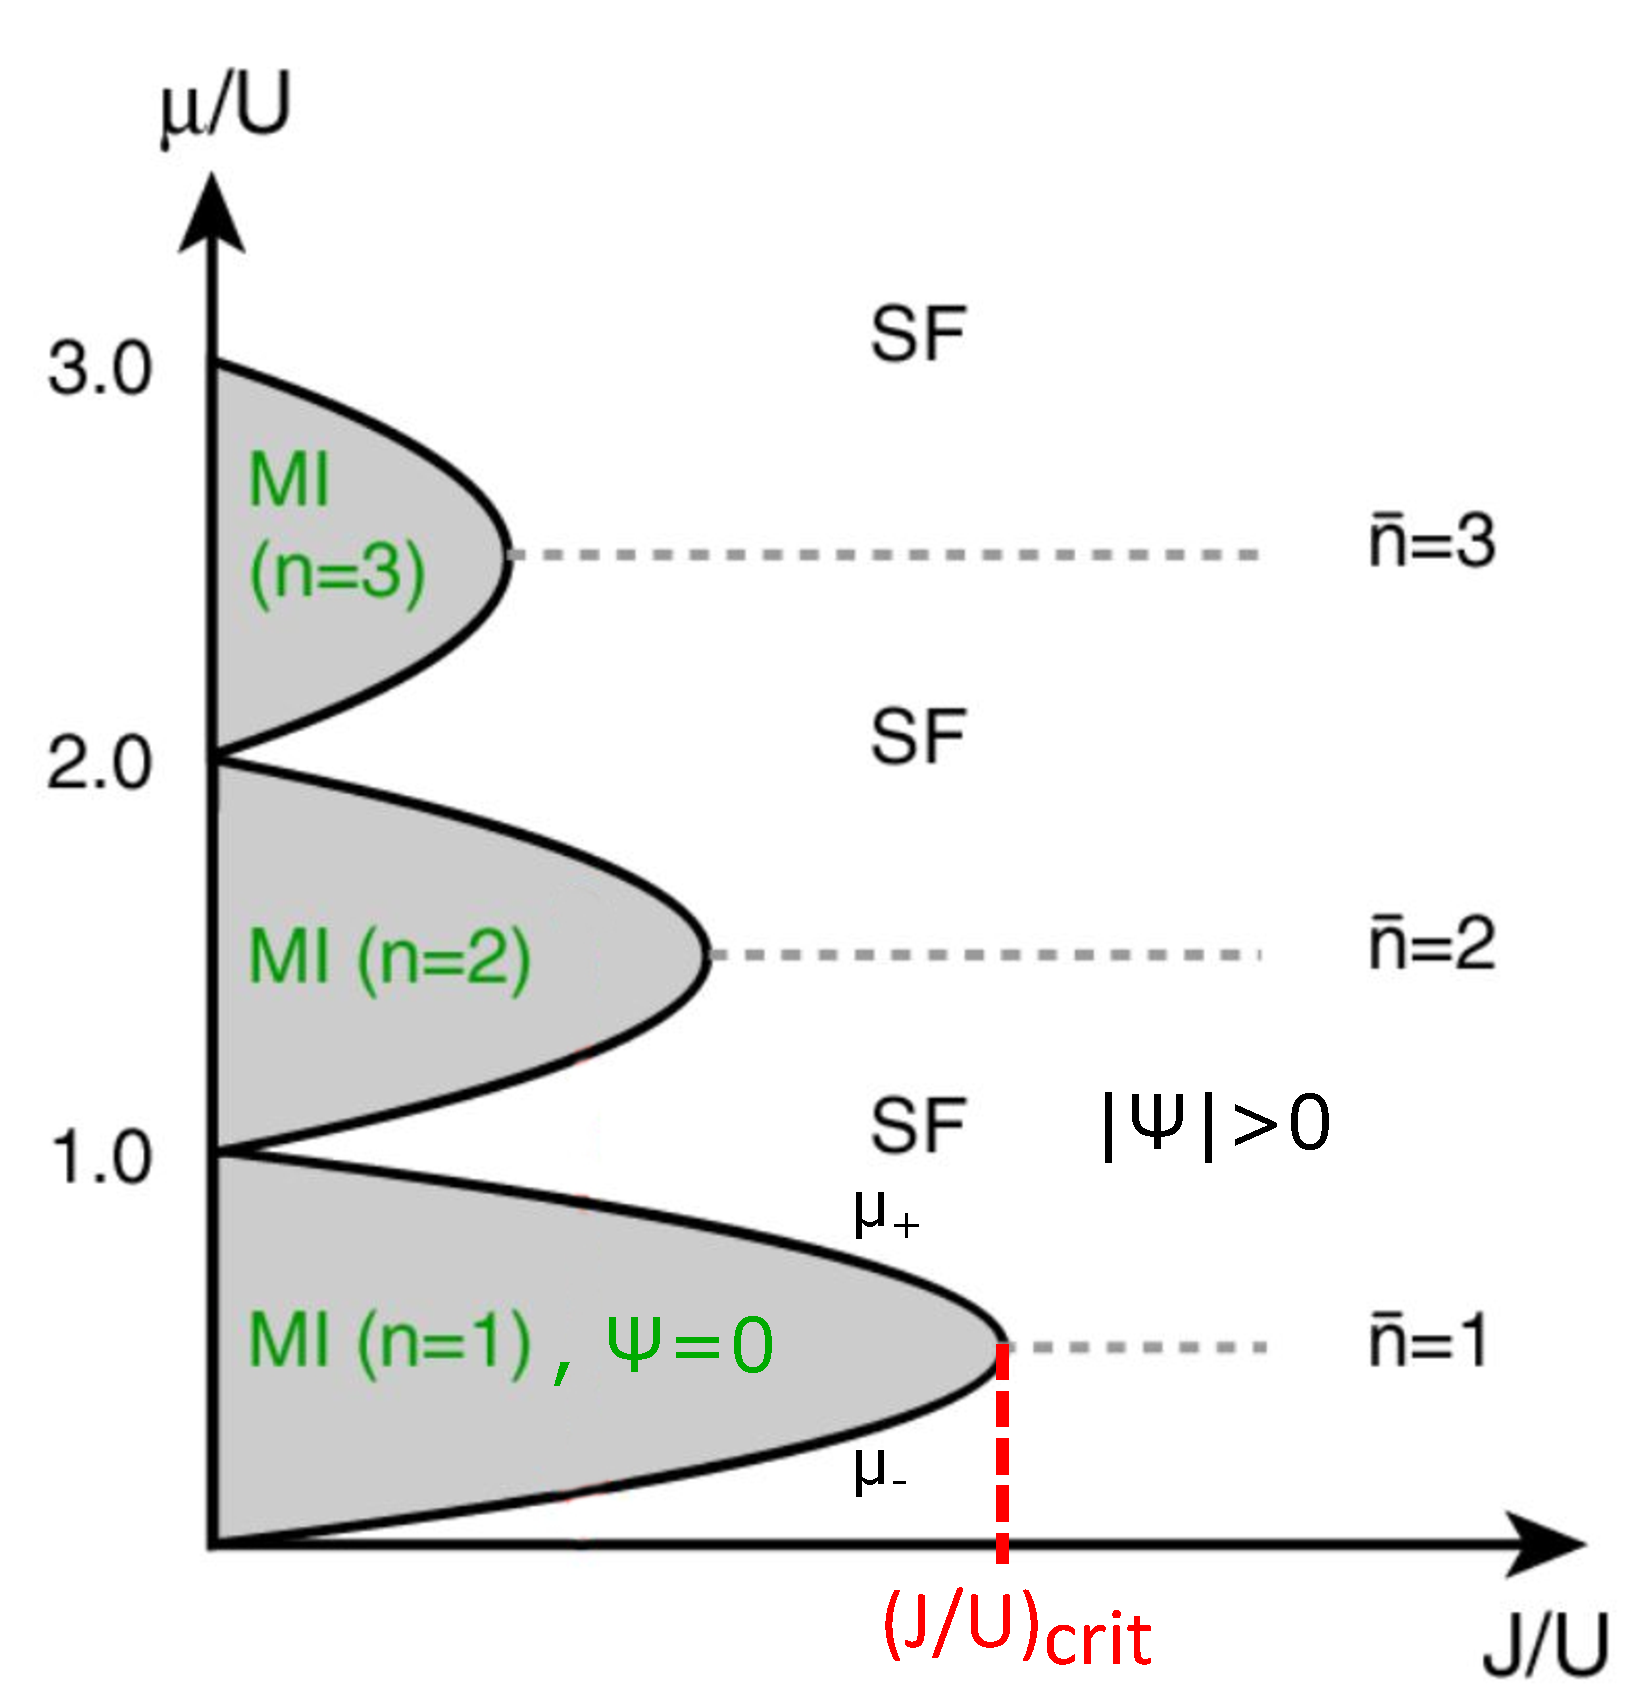
\includegraphics[width = 0.5\textwidth]{Figures/SFMottPhase.pdf}
	\caption{Phase diagram of Bose-Hubbard model for $T = 0$. Grey areas mark the Mott-insulator phase for different number of particles per site. The Mott-insulator is incompressible, whereby $\partial n / \partial \mu = 0$. Meanwhile white regions mark the superfluid phase. \cite{greiner}}
	\label{fig:MeanFieldPhaseDiagram}
\end{figure}
A better understanding of the results can be obtained by examining figure \ref{fig:MeanFieldPhaseDiagram}, which displays the mean-field phase diagram of the Bose-Hubbard model. 
The $\mu_{\pm}$ curves enclose the region where the system is in the Mott-insulating phase. $(1/\bar{U})_{crit} = (J/U)_{crit}$ can be read off the graph from the point where the two curves $\mu_{\pm}$ meet. No number fluctuations take place in the Mott-insulator, whereby the particle number per site is well defined. As the chemical potential increases, each site can accommodate more particles as long as the increase in chemical potential compensates the increased energy due to interactions between the particles.

The mean-field solution of the Bose-Hubbard model is only an approximation, which proves quite inaccurate for one dimension. This is obvious when comparing the critical ratio for the mean-field approach, $\left( U/J \right)_{crit}^{MF,1D} = 11.66$, with numerical results computed using the DMRG method, $\left( U/J \right)_{crit}^{DMRG,1D} = 3.37$, \cite{Kuhner2000}. Nevertheless, the mean-field gives a good intuitive feeling of the physics taking place and how one can describe them without resorting to diagonalizing the full Hamiltonian.